\documentclass[letterpaper,12pt]{article}
\usepackage{graphicx} % Required for inserting images
\usepackage{amsmath}

\title{Constant Acceleration Lab}
\author{Lennon McLean}
\date{September 24, 2024}

\begin{document}

\maketitle

\section*{\underline{Purpose}}
The purpose of this lab is to understand how the position and velocity of a dynamics cart change when it is under constant acceleration.

\section*{\underline{Materials}}
\begin{itemize}
    \item C-clamp
    \item Ramp
    \item Masking Tape
    \item Recording Tape
    \item Ruler
    \item Dynamics Cart
    \item Spark Timer
\end{itemize}

\section*{\underline{Procedure}}
Refer to Wardell, J. (2024). "Lab - Motion Down a Ramp". Handout.

\section*{\underline{Observations and Results}}
\hspace*{-2.5cm}
\begin{tabular}{|p{2cm}|p{3cm}|p{3cm}|p{3cm}|p{3cm}|p{2cm}|}
    \hline
    Time, $t$ (s) & Displacement, $\Delta d$ (cm) [down ramp] & Displacement, $\Delta d$ (m) [down ramp] & Position, $d$ (m) & Velocity, $v$ (m/s) [down ramp] & Half time (s) \\ \hline
    0 &  &  &  &  &  \\ \hline
    0.1 & 1.1 & 0.011 & 0.011 & 0.11 & 0.05 \\ \hline
    0.2 & 2.2 & 0.022 & 0.033 & 0.22 & 0.15 \\ \hline
    0.3 & 4.2 & 0.042 & 0.075 & 0.42 & 0.25 \\ \hline
    0.4 & 6.2 & 0.062 & 0.137 & 0.62 & 0.35 \\ \hline
    0.5 & 8.9 & 0.089 & 0.226 & 0.89 & 0.45 \\ \hline
    0.6 & 10.2 & 0.102 & 0.328 & 1.02 & 0.55 \\ \hline
\end{tabular}
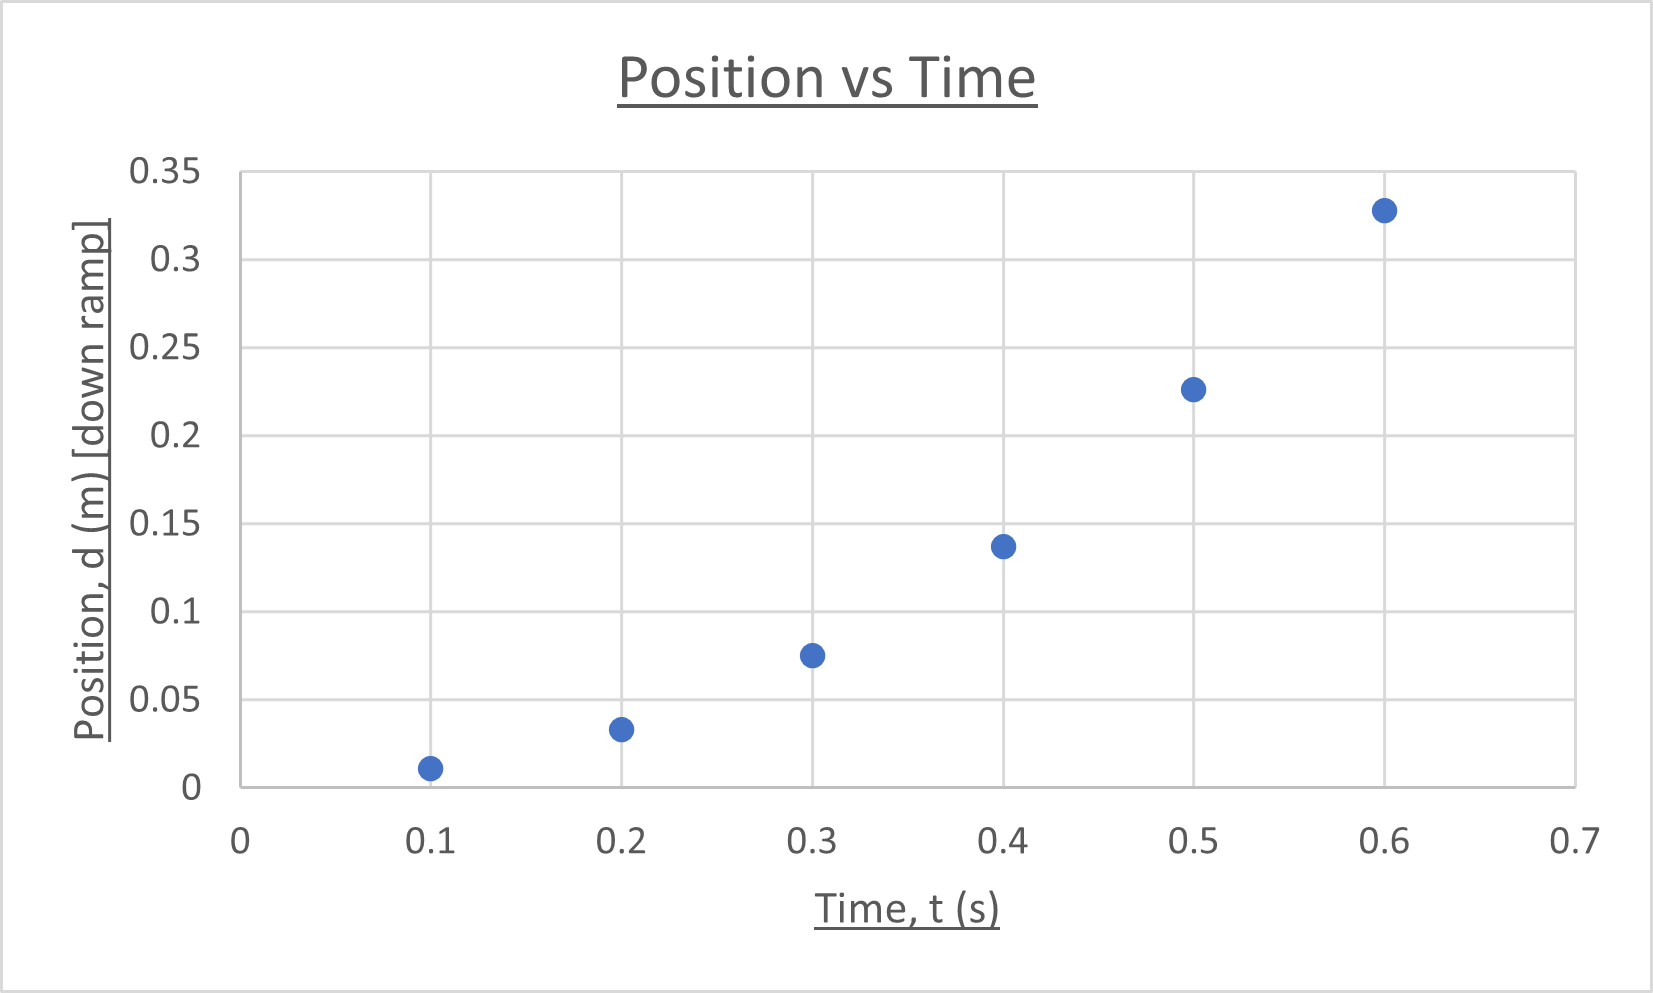
\includegraphics{pos-time}

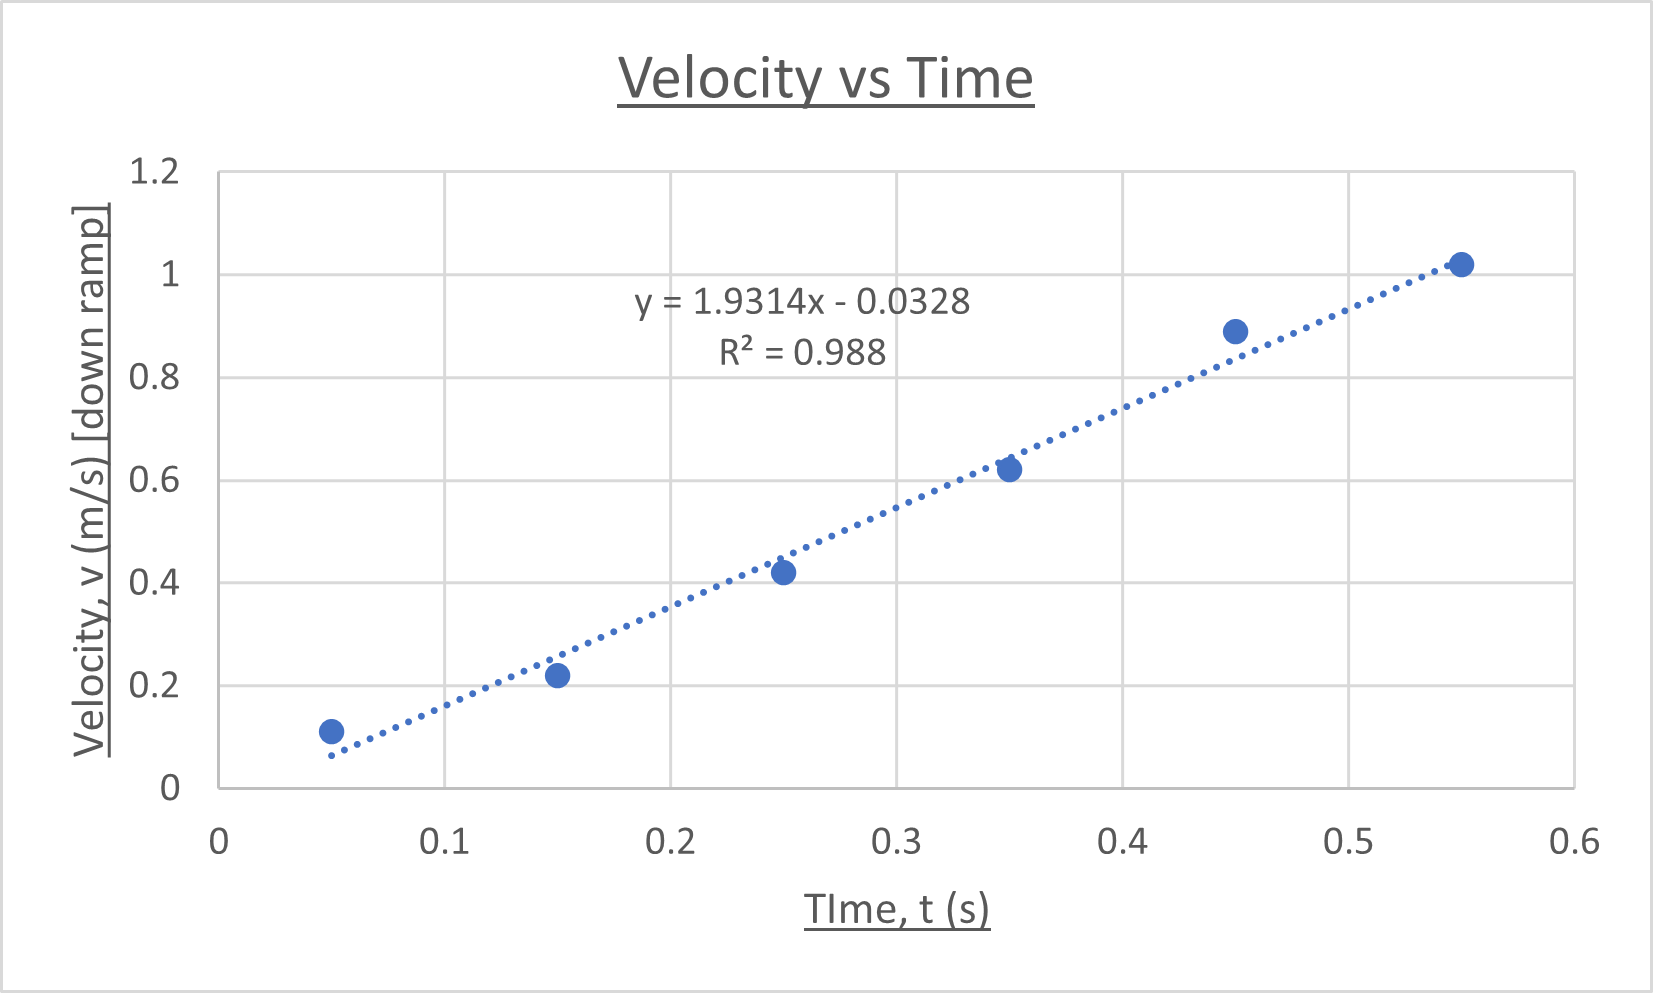
\includegraphics{vel-time}

\section*{\underline{Analysis}}
Initial velocity, acceleration, and time values are taken from the v-t graph.
\begin{align*}
    \Delta d&=v\Delta t+\frac{1}{2}a(\Delta t)^2\\
    \Delta d&=-0.03\frac{m}{s}\cdot0.6s+\frac{1}{2}\cdot1.93\frac{m}{s^2}\cdot(0.6s)^2\\
    \Delta d&=0.33m\text{ [down ramp]}
\end{align*}
This matches the final position returned by Excel in the observations table.

\section*{\underline{Discussion}}
\begin{enumerate}
    \item \begin{enumerate}
        \item As time increases, the slope of the tangent line on the position-time graph increases linearly.
        \item As time increases, the slope of the best-fit line on the velocity-time graph stays constant.
        \item The slope of the velocity-time graph line remains constant since the acceleration on the cart is constant. The slope of the tangent line of the position-time graph increases because the velocity increases, and the slope of the tangent line IS the velocity.
    \end{enumerate}
    \item According to the graph made by Excel, the acceleration of the cart is 1.93 $\frac{m}{s^2}$ [down ramp].
    \item If the data points were plotted at the end time for each interval, the entire graph would have been shifted to the right, giving the impression that the cart started moving later than it really did.
    \item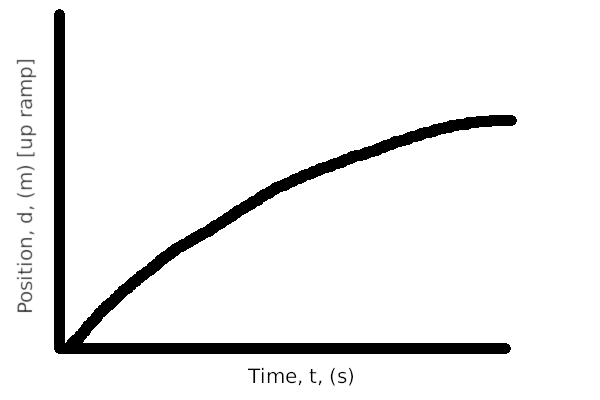
\includegraphics[width=6cm]{p-t}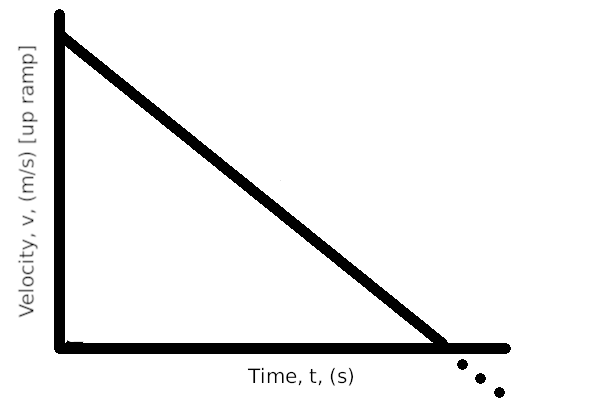
\includegraphics[width=6cm]{v-t}
    \item Possible sources of error in 4. include possible slack or motion of the paper tape during the experiment, and imprecision in measuring the dots on the tape.
\end{enumerate}

\section*{\underline{Conclusion}}
In conclusion, when a dynamics cart (or any object) is placed an the top of a ramp, it undergoes constant acceleration due to gravity. This causes the velocity of the cart to increase linearly, which in turn causes the position of the cart relative to the start to increase quadratically.

\end{document}